\documentclass{scrreprt}

\usepackage{aligned-overset}
\usepackage{amsmath}
\usepackage{amsthm}
\usepackage{amssymb}
\usepackage{bm}
\usepackage[inline, shortlabels]{enumitem}
\usepackage{hyperref}
\usepackage[utf8]{inputenc}
\usepackage{listings}
\usepackage{multicol}
\usepackage{mathtools}
\usepackage{pdflscape}
\usepackage{physics}
\usepackage{polynom}
\usepackage{tabularx}
\usepackage[table]{xcolor}
\usepackage{titling}
\usepackage{fancyhdr}
\usepackage{xfrac}
\usepackage{pgfplots}

\pgfplotsset{compat = newest}
\usepgfplotslibrary{fillbetween}
\usetikzlibrary{arrows, arrows.meta}
\usetikzlibrary{calc}
\usetikzlibrary{patterns}

\author{Karsten Lehmann}
\date{WiSe 2024/25}
\title{Übungsblatt 14\\INF-B-110, Diskrete Strukturen}

\setlength{\parindent}{0pt}

\setlength{\headheight}{26pt}
\pagestyle{fancy}
\fancyhf{}
\lhead{\thetitle}
\rhead{\theauthor}
\lfoot{\thedate}
\rfoot{Seite \thepage}

\begin{document}
\paragraph{Ü 14.1}

Welche der folgenden, durch unbeschriftete Diagramme gegebenen Graphen sind
planar?
Geben Sie entweder eine Zeichnung an, oder geben Sie an, wie Sie $K_{3, 3}$ oder
$K_5$ als Minor erhalten.

\begin{minipage}{0.25\textwidth}
  \begin{tikzpicture}
    \node[circle, draw, inner sep=0pt, minimum size=1mm] (1) at (0,0) {};
    \node[circle, draw, inner sep=0pt, minimum size=1mm] (2) at (1,0) {};
    \node[circle, draw, inner sep=0pt, minimum size=1mm] (3) at (2,-1) {};
    \node[circle, draw, inner sep=0pt, minimum size=1mm] (4) at (2,-2) {};
    \node[circle, draw, inner sep=0pt, minimum size=1mm] (5) at (1,-3) {};
    \node[circle, draw, inner sep=0pt, minimum size=1mm] (6) at (0,-3) {};
    \node[circle, draw, inner sep=0pt, minimum size=1mm] (7) at (-1,-2) {};
    \node[circle, draw, inner sep=0pt, minimum size=1mm] (8) at (-1,-1) {};

    \draw (1) -- (2) -- (3) -- (4) -- (5) -- (6) -- (7) -- (8) -- (1);
    \draw (1) -- (5);
    \draw (2) -- (6);
    \draw (3) -- (7);
    \draw (4) -- (8);
  \end{tikzpicture}
\end{minipage}
\begin{minipage}{0.25\textwidth}
  \begin{tikzpicture}
    \node[circle, draw, inner sep=0pt, minimum size=1mm] (1) at (0,0) {};
    \node[circle, draw, inner sep=0pt, minimum size=1mm] (2) at (1,0) {};
    \node[circle, draw, inner sep=0pt, minimum size=1mm] (3) at (2,-1) {};
    \node[circle, draw, inner sep=0pt, minimum size=1mm] (4) at (2,-2) {};
    \node[circle, draw, inner sep=0pt, minimum size=1mm] (5) at (1,-3) {};
    \node[circle, draw, inner sep=0pt, minimum size=1mm] (6) at (0,-3) {};
    \node[circle, draw, inner sep=0pt, minimum size=1mm] (7) at (-1,-2) {};
    \node[circle, draw, inner sep=0pt, minimum size=1mm] (8) at (-1,-1) {};

    \draw (1) -- (2) -- (3) -- (4) -- (5) -- (6) -- (7) -- (8) -- (1);
    \draw (1) -- (3) -- (5) -- (7) -- (1);
    \draw (2) -- (6);
    \draw (4) -- (8);
  \end{tikzpicture}
\end{minipage}
\begin{minipage}{0.25\textwidth}
  \begin{tikzpicture}
    \node[circle, draw, inner sep=0pt, minimum size=1mm] (1) at (-0.5,0) {};
    \node[circle, draw, inner sep=0pt, minimum size=1mm] (2) at (1,0) {};
    \node[circle, draw, inner sep=0pt, minimum size=1mm] (3) at (-1,-3) {};
    \node[circle, draw, inner sep=0pt, minimum size=1mm] (4) at (-0.5,-3) {};
    \node[circle, draw, inner sep=0pt, minimum size=1mm] (5) at (0,-3) {};
    \node[circle, draw, inner sep=0pt, minimum size=1mm] (6) at (0.5,-3) {};
    \node[circle, draw, inner sep=0pt, minimum size=1mm] (7) at (1,-3) {};
    \node[circle, draw, inner sep=0pt, minimum size=1mm] (8) at (1.5,-3) {};

    \draw (1) -- (3) -- (2);
    \draw (1) -- (4) -- (2);
    \draw (1) -- (5) -- (2);
    \draw (1) -- (6) -- (2);
    \draw (1) -- (7) -- (2);
    \draw (1) -- (8) -- (2);
    \draw (1) -- (2);
    \draw (3) -- (4) -- (5) -- (6) -- (7) -- (8);
  \end{tikzpicture}
\end{minipage}
\begin{minipage}{0.25\textwidth}
  \begin{tikzpicture}
    \node[circle, draw, inner sep=0pt, minimum size=1mm] (1) at (-1,0) {};
    \node[circle, draw, inner sep=0pt, minimum size=1mm] (2) at (1,0) {};
    \node[circle, draw, inner sep=0pt, minimum size=1mm] (3) at (1.5,0) {};
    \node[circle, draw, inner sep=0pt, minimum size=1mm] (4) at (2,0) {};
    \node[circle, draw, inner sep=0pt, minimum size=1mm] (5) at (2,-1.5) {};
    \node[circle, draw, inner sep=0pt, minimum size=1mm] (6) at (2,-3) {};
    \node[circle, draw, inner sep=0pt, minimum size=1mm] (7) at (1,-3) {};
    \node[circle, draw, inner sep=0pt, minimum size=1mm] (8) at (0,-3) {};
    \node[circle, draw, inner sep=0pt, minimum size=1mm] (9) at (-1,-3) {};
    \node[circle, draw, inner sep=0pt, minimum size=1mm] (10) at (-1,-2) {};

    \draw (1) -- (2) -- (3) -- (4) -- (5) -- (6) -- (7) -- (8) -- (9) -- (10) -- (1);
    \draw (2) -- (7);
    \draw (3) -- (8);
    \draw (5) -- (10);
  \end{tikzpicture}
\end{minipage}

\vspace{0.5cm}

Prüfen Sie für die planaren Graphen die Eulersche Polyederformel.

\subparagraph{Lsg.} Es sind

\begin{minipage}{0.5\textwidth}
  \begin{tikzpicture}
    \node[circle, draw, fill, inner sep=0pt, minimum size=1mm] (1) at (0,0) {};
    \node[circle, draw, fill, inner sep=0pt, minimum size=1mm] (2) at (2,0) {};
    \node[circle, draw, fill, inner sep=0pt, minimum size=1mm] (3) at (0,-1) {};
    \node[circle, draw, fill, inner sep=0pt, minimum size=1mm] (4) at (2,-1) {};
    \node[circle, draw, fill, inner sep=0pt, minimum size=1mm] (5) at (0,-2) {};
    \node[circle, draw, fill, inner sep=0pt, minimum size=1mm] (6) at (2,-2) {};

    \draw (1) -- (2) -- (5) -- (6) -- (1) -- (4) -- (3) -- (2);
    \draw (6) -- (3);
    \draw (5) -- (4);

    \node at (0, -2.5) {$K_{3, 3}$};
  \end{tikzpicture}
\end{minipage}
\begin{minipage}{0.5\textwidth}
  \begin{tikzpicture}
    \node[circle, draw, fill, inner sep=0pt, minimum size=1mm] (1) at (0,1) {};
    \node[circle, draw, fill, inner sep=0pt, minimum size=1mm] (2) at ($({-0.5*sqrt(0.5*(5+sqrt(5)))}, {sqrt(5)/4 - 0.25})$) {};
    \node[circle, draw, fill, inner sep=0pt, minimum size=1mm] (3) at ($({-0.5*sqrt(0.5*(5-sqrt(5)))}, {-0.25 - sqrt(5)/4})$) {};
    \node[circle, draw, fill, inner sep=0pt, minimum size=1mm] (4) at ($({0.5*sqrt(0.5*(5-sqrt(5)))}, {-0.25 - sqrt(5)/4})$) {};
    \node[circle, draw, fill, inner sep=0pt, minimum size=1mm] (5) at ($({0.5*sqrt(0.5*(5+sqrt(5)))}, {sqrt(5)/4 - 0.25})$) {};

    \draw (1) -- (2) -- (3) -- (4) -- (5) -- (1) -- (3) -- (5) -- (2) -- (4) -- (1);

    \node at (0, -1.5) {$K_5$};
  \end{tikzpicture}
\end{minipage}

Nun ist für den ersten Graphen $K_{3, 3}$ ein Minor.

\begin{minipage}{0.25\textwidth}
  \begin{tikzpicture}
    \node[circle, draw, inner sep=0pt, minimum size=1mm] (1) at (0,0) {};
    \node[circle, draw, inner sep=0pt, minimum size=1mm] (2) at (1,0) {};
    \node[circle, draw, inner sep=0pt, minimum size=1mm] (3) at (2,-1) {};
    \node[circle, draw, inner sep=0pt, minimum size=1mm] (4) at (2,-2) {};
    \node[circle, draw, inner sep=0pt, minimum size=1mm] (5) at (1,-3) {};
    \node[circle, draw, inner sep=0pt, minimum size=1mm] (6) at (0,-3) {};
    \node[circle, draw, inner sep=0pt, minimum size=1mm] (7) at (-1,-2) {};
    \node[circle, draw, inner sep=0pt, minimum size=1mm] (8) at (-1,-1) {};

    \draw (1) -- (2) -- (3) -- (4) -- (5) -- (6) -- (7) -- (8) -- (1);
    \draw (1) -- (5);
    \draw (2) -- (6);
    \draw (3) -- (7);
    \draw (4) -- (8);
  \end{tikzpicture}
\end{minipage}
\begin{minipage}{0.25\textwidth}
  \begin{tikzpicture}
    \node[circle, draw, inner sep=0pt, minimum size=1mm] (1) at (0,0) {};
    \node[circle, draw, inner sep=0pt, minimum size=1mm] (2) at (1,0) {};
    \node[circle, draw, inner sep=0pt, minimum size=1mm] (3) at (2,-1) {};
    \node[circle, draw, inner sep=0pt, minimum size=1mm] (4) at (2,-2) {};
    \node[circle, draw, inner sep=0pt, minimum size=1mm] (5) at (1,-3) {};
    \node[circle, draw, inner sep=0pt, minimum size=1mm] (6) at (0,-3) {};
    \node[circle, draw, inner sep=0pt, minimum size=1mm] (7) at (-1,-2) {};

    \draw (1) -- (2) -- (3) -- (4) -- (5) -- (6) -- (7) -- (1);
    \draw (1) -- (5);
    \draw (2) -- (6);
    \draw (3) -- (7);
    \draw (4) -- (1);
  \end{tikzpicture}
\end{minipage}
\begin{minipage}{0.25\textwidth}
  \begin{tikzpicture}
    \node[circle, draw, inner sep=0pt, minimum size=1mm] (1) at (0,0) {};
    \node[circle, draw, inner sep=0pt, minimum size=1mm] (2) at (1,0) {};
    \node[circle, draw, inner sep=0pt, minimum size=1mm] (3) at (2,-1) {};
    \node[circle, draw, inner sep=0pt, minimum size=1mm] (5) at (1,-3) {};
    \node[circle, draw, inner sep=0pt, minimum size=1mm] (6) at (0,-3) {};
    \node[circle, draw, inner sep=0pt, minimum size=1mm] (7) at (-1,-2) {};

    \draw (1) -- (2) -- (3) -- (5) -- (6) -- (7) -- (1);
    \draw (1) -- (5);
    \draw (2) -- (6);
    \draw (3) -- (7);
  \end{tikzpicture}
\end{minipage}
\begin{minipage}{0.25\textwidth}
  \begin{tikzpicture}
    \node[circle, draw, inner sep=0pt, minimum size=1mm] (1) at (0,0) {};
    \node[circle, draw, inner sep=0pt, minimum size=1mm] (2) at (1,0) {};
    \node[circle, draw, inner sep=0pt, minimum size=1mm] (3) at (2,-1) {};
    \node[circle, draw, inner sep=0pt, minimum size=1mm] (5) at (1,-3) {};
    \node[circle, draw, inner sep=0pt, minimum size=1mm] (6) at (0,-3) {};
    \node[circle, draw, inner sep=0pt, minimum size=1mm] (7) at (-1,-2) {};

    \draw (1) -- (2) -- (7) -- (5) -- (6) -- (3) -- (1);
    \draw (1) -- (5);
    \draw (2) -- (6);
    \draw (3) -- (7);
  \end{tikzpicture}
\end{minipage}

Der zweite Graph ist planar:

\begin{minipage}{0.3\textwidth}
  \begin{tikzpicture}
    \node[circle, draw, inner sep=0pt, minimum size=1mm] (1) at (0,0) {};
    \node[circle, draw, inner sep=0pt, minimum size=1mm] (2) at (1,0) {};
    \node[circle, draw, inner sep=0pt, minimum size=1mm] (3) at (2,-1) {};
    \node[circle, draw, inner sep=0pt, minimum size=1mm] (4) at (2,-2) {};
    \node[circle, draw, inner sep=0pt, minimum size=1mm] (5) at (1,-3) {};
    \node[circle, draw, inner sep=0pt, minimum size=1mm] (6) at (0,-3) {};
    \node[circle, draw, inner sep=0pt, minimum size=1mm] (7) at (-1,-2) {};
    \node[circle, draw, inner sep=0pt, minimum size=1mm] (8) at (-1,-1) {};

    \draw (1) -- (2) -- (3) -- (4) -- (5) -- (6) -- (7) -- (8) -- (1);
    \draw (1) -- (3) -- (5) -- (7) -- (1);
    \draw (2) -- (6);
    \draw (4) -- (8);
  \end{tikzpicture}
\end{minipage}
\begin{minipage}{0.3\textwidth}
  \begin{tikzpicture}
    \node[circle, draw, inner sep=0pt, minimum size=1mm] (1) at (0,0) {};
    \node[circle, draw, inner sep=0pt, minimum size=1mm] (2) at (-0.5,1) {};
    \node[circle, draw, inner sep=0pt, minimum size=1mm] (3) at (2,-1) {};
    \node[circle, draw, inner sep=0pt, minimum size=1mm] (4) at (2,-2) {};
    \node[circle, draw, inner sep=0pt, minimum size=1mm] (5) at (1,-3) {};
    \node[circle, draw, inner sep=0pt, minimum size=1mm] (6) at (-2,-3) {};
    \node[circle, draw, inner sep=0pt, minimum size=1mm] (7) at (-1,-2) {};
    \node[circle, draw, inner sep=0pt, minimum size=1mm] (8) at (-1,-1) {};

    \draw (1) -- (2) -- (3) -- (4) -- (5) -- (6) -- (7) -- (8) -- (1);
    \draw (1) -- (3) -- (5) -- (7) -- (1);
    \draw (2) -- (6);
    \draw (4) -- (8);
  \end{tikzpicture}
\end{minipage}
\begin{minipage}{0.3\textwidth}
  \begin{tikzpicture}
    \node[circle, draw, inner sep=0pt, minimum size=1mm] (1) at (0,0) {};
    \node[circle, draw, inner sep=0pt, minimum size=1mm] (2) at (-0.5,1) {};
    \node[circle, draw, inner sep=0pt, minimum size=1mm] (3) at (2,-1) {};
    \node[circle, draw, inner sep=0pt, minimum size=1mm] (4) at (1,-2) {};
    \node[circle, draw, inner sep=0pt, minimum size=1mm] (5) at (1,-3) {};
    \node[circle, draw, inner sep=0pt, minimum size=1mm] (6) at (-2,-3) {};
    \node[circle, draw, inner sep=0pt, minimum size=1mm] (7) at (-1,-2) {};
    \node[circle, draw, inner sep=0pt, minimum size=1mm] (8) at (0,-1) {};

    \draw (1) -- (2) -- (3) -- (4) -- (5) -- (6) -- (7) -- (8) -- (1);
    \draw (1) -- (3) -- (5) -- (7) -- (1);
    \draw (2) -- (6);
    \draw (4) -- (8);
  \end{tikzpicture}
\end{minipage}

Nun hat der zweite Graph $8$ Ecken, $14$ Kanten und $8$ Flächen (die Außenfläche
zählt mit).
Die Eulersche Polyederformel besagt \emph{``Es sei $\qty\big(V, E)$ ein
  zusammenhängender ebener Graph mit $n$ Ecken, $m$ Kanten und $l$ Flächen.
  Dann gilt $n - m + l = 2$''}.
Und tatsächlich ist
\[
  8 - 14 + 8 = 2.
\]

\newpage
Der dritte Graph ist planar

\begin{minipage}{0.25\textwidth}
  \begin{tikzpicture}
    \node[circle, draw, inner sep=0pt, minimum size=1mm] (1) at (-0.5,0) {};
    \node[circle, draw, inner sep=0pt, minimum size=1mm] (2) at (1,0) {};
    \node[circle, draw, inner sep=0pt, minimum size=1mm] (3) at (-1,-3) {};
    \node[circle, draw, inner sep=0pt, minimum size=1mm] (4) at (-0.5,-3) {};
    \node[circle, draw, inner sep=0pt, minimum size=1mm] (5) at (0,-3) {};
    \node[circle, draw, inner sep=0pt, minimum size=1mm] (6) at (0.5,-3) {};
    \node[circle, draw, inner sep=0pt, minimum size=1mm] (7) at (1,-3) {};
    \node[circle, draw, inner sep=0pt, minimum size=1mm] (8) at (1.5,-3) {};

    \draw (1) -- (3) -- (2);
    \draw (1) -- (4) -- (2);
    \draw (1) -- (5) -- (2);
    \draw (1) -- (6) -- (2);
    \draw (1) -- (7) -- (2);
    \draw (1) -- (8) -- (2);
    \draw (1) -- (2);
    \draw (3) -- (4) -- (5) -- (6) -- (7) -- (8);
  \end{tikzpicture}
\end{minipage}
\begin{minipage}{0.25\textwidth}
  \begin{tikzpicture}
    \node[circle, draw, inner sep=0pt, minimum size=1mm] (1) at (2,0) {};
    \node[circle, draw, inner sep=0pt, minimum size=1mm] (2) at (2,-3) {};
    \node[circle, draw, inner sep=0pt, minimum size=1mm] (3) at (-1,-1.5) {};
    \node[circle, draw, inner sep=0pt, minimum size=1mm] (4) at (-0.5,-1.5) {};
    \node[circle, draw, inner sep=0pt, minimum size=1mm] (5) at (0,-1.5) {};
    \node[circle, draw, inner sep=0pt, minimum size=1mm] (6) at (0.5,-1.5) {};
    \node[circle, draw, inner sep=0pt, minimum size=1mm] (7) at (1,-1.5) {};
    \node[circle, draw, inner sep=0pt, minimum size=1mm] (8) at (1.5,-1.5) {};

    \draw (1) -- (3) -- (2);
    \draw (1) -- (4) -- (2);
    \draw (1) -- (5) -- (2);
    \draw (1) -- (6) -- (2);
    \draw (1) -- (7) -- (2);
    \draw (1) -- (8) -- (2);
    \draw (1) -- (2);
    \draw (3) -- (4) -- (5) -- (6) -- (7) -- (8);
  \end{tikzpicture}
\end{minipage}

Nun hat der Graph $8$ Ecken, $13$ Kanten und $12$ Flächen.
Wieder ist
\[
  8 - 18 + 12 = 2
\]

Der vierte Graph hat wieder $K_{3, 3}$ als Minor:

\begin{minipage}{0.25\textwidth}
  \begin{tikzpicture}
    \node[circle, draw, inner sep=0pt, minimum size=1mm] (1) at (-1,0) {};
    \node[circle, draw, inner sep=0pt, minimum size=1mm] (2) at (1,0) {};
    \node[circle, draw, inner sep=0pt, minimum size=1mm] (3) at (1.5,0) {};
    \node[circle, draw, inner sep=0pt, minimum size=1mm] (4) at (2,0) {};
    \node[circle, draw, inner sep=0pt, minimum size=1mm] (5) at (2,-1.5) {};
    \node[circle, draw, inner sep=0pt, minimum size=1mm] (6) at (2,-3) {};
    \node[circle, draw, inner sep=0pt, minimum size=1mm] (7) at (1,-3) {};
    \node[circle, draw, inner sep=0pt, minimum size=1mm] (8) at (0,-3) {};
    \node[circle, draw, inner sep=0pt, minimum size=1mm] (9) at (-1,-3) {};
    \node[circle, draw, inner sep=0pt, minimum size=1mm] (10) at (-1,-2) {};

    \draw (1) -- (2) -- (3) -- (4) -- (5) -- (6) -- (7) -- (8) -- (9) -- (10) -- (1);
    \draw (2) -- (7);
    \draw (3) -- (8);
    \draw (5) -- (10);
  \end{tikzpicture}
\end{minipage}
\begin{minipage}{0.25\textwidth}
  \begin{tikzpicture}
    \node[circle, draw, inner sep=0pt, minimum size=1mm] (2) at (1,0) {};
    \node[circle, draw, inner sep=0pt, minimum size=1mm] (3) at (1.5,0) {};
    \node[circle, draw, inner sep=0pt, minimum size=1mm] (5) at (2,-1.5) {};
    \node[circle, draw, inner sep=0pt, minimum size=1mm] (7) at (1,-3) {};
    \node[circle, draw, inner sep=0pt, minimum size=1mm] (8) at (0,-3) {};
    \node[circle, draw, inner sep=0pt, minimum size=1mm] (10) at (-1,-2) {};

    \draw (2) -- (3)  -- (5) -- (7) -- (8) -- (10) -- (2);
    \draw (2) -- (7);
    \draw (3) -- (8);
    \draw (5) -- (10);
  \end{tikzpicture}
\end{minipage}
\begin{minipage}{0.25\textwidth}
  \begin{tikzpicture}
    \node[circle, draw, inner sep=0pt, minimum size=1mm] (2) at (0,0) {};
    \node[circle, draw, inner sep=0pt, minimum size=1mm] (3) at (2,0) {};
    \node[circle, draw, inner sep=0pt, minimum size=1mm] (5) at (0,-1.5) {};
    \node[circle, draw, inner sep=0pt, minimum size=1mm] (7) at (2,-3) {};
    \node[circle, draw, inner sep=0pt, minimum size=1mm] (8) at (0,-3) {};
    \node[circle, draw, inner sep=0pt, minimum size=1mm] (10) at (2,-1.5) {};

    \draw (2) -- (3)  -- (5) -- (7) -- (8) -- (10) -- (2);
    \draw (2) -- (7);
    \draw (3) -- (8);
    \draw (5) -- (10);
  \end{tikzpicture}
\end{minipage}

\paragraph{Ü 14.2} Ermitteln Sie, wie viele Flächen ein planarer Graph
$G = \qty\big(V, E)$ haben kann, wenn $\abs{V} = 10$ ist und alle Knoten
den Grad 3 haben.

\subparagraph{Lsg.} Jede Kante in dem Graphen erhöht den Grad von 2 Knoten um
eins.
Dementsprechend hat der Graph $\frac{3 \cdot 10}{2} = 15$ Kanten.
Nach der Eulerschen Polyederformel ist nun
\[
  10 - 15 + l = 2
\]
und der Graph hat $l = 7$ Flächen.

\paragraph{Ü 14.3} Finden Sie eine endliche Menge $\mathcal{F}$, so dass gilt:
Ein Graph $G$ ist genau dann ein Wald, wenn $G$ keinen Graphen aus $\mathcal{F}$
als Minoren hat.

\subparagraph{Lsg.} Ein Wald ist ein nicht notwendigerweise zusammenhängender
Graph ohne Kreise.

Vermutung $\mathcal{F} = \qty\big{C_3}$.

\newpage
\paragraph{Ü 14.4} Die Oberfläche eines Fußballs ist aus Fünfecken und
Sechsecken zusammengesetzt, sie kann durch einen Ebenen Graphen
$\qty\big(V, E, i)$ mit 60 Knoten dargestellt werden, in dem sich in jedem Knoten
genau zwei Sechsecke und ein Fünfeck treffen.
\begin{enumerate}[(a)]
\item Berechnen Sie die Kantenanzahl des ebenen Graphen $\qty\big(V, E, i)$ und
  bestimmen Sie die Anzahl der Fünfeckflächen und der Sechseckflächen dieses
  Graphen.

  \subparagraph{Lsg.} Es hat jeder Knoten den Grad 3 und der Graph somit
  $\frac{3 \cdot 60}{2} = 90$ Kanten.

  Nun ist hat der Graph nach der Eulerschen Polyederformel
  \[
    60 - 90 + l = 2
  \]
  insgesamt $l = 32$ Flächen.

  Weiter treffen sich in jedem Knoten genau zwei Sechsecke und ein Fünfeck.
  Folglich ist jeder Knoten teil eines Fünfecks und zwei paarweise verschiedene
  Fünfecke haben keine gemeinsamen Knoten.

  Dementsprechend hat der Graph $\frac{60}{5} = 12$ Fünfecke und 20 Sechsecke.

  \textbf{Alternativ nach der Übung:} Sei $l_5$ die Anzahl der Fünfecke und
  $l_6$ die Anzahl der Sechsecke.
  Dann ist $l_5 + l_6 = 32$.

  Außerdem hat ein Fünfeck 5 Kanten und ein Seckseck 6 Kanten, somit ist
  $5 \cdot l_5 + 6 \cdot l_6 = 2 \cdot m = 3 \cdot n$.

  Das ist ein Gleichungssystem mit 2 Gleichungen und zwei unbekannten, somit
  schnell lösbar.

\item Ist es möglich, einen Fußball zu schaffen, dessen Oberfläche nur aus
  Fünfecken bzw. nur aus Sechsecken besteht, wenn in jeder Ecke genau drei
  Flächen zusammentreffen sollen?

  \subparagraph{Lsg.} Angenommen der Fußball mit Fünf- oder Sechsecken hat $n$
  Knoten, dann hat er da jeder Knoten den Grad $3$ hat $\frac{3 \cdot n}{2}$
  Kanten.

  Weiter hat ein Fünfeck 5 Kanten und jede Kante ist Teil von 2 Fünfecken,
  das heißt ein Fußball mit $n$ Ecken hat $\frac{3 \cdot n}{5}$ Flächen.
  \[
    n - \frac{3 \cdot n}{2} + \frac{3 \cdot n}{5} =
    \frac{10n}{10} - \frac{15n}{10} + \frac{6 \cdot n}{10}
    = \frac{n}{10} = 2 = \frac{20}{2}
  \]
  Somit existiert ein Fußball mit $20$ Ecken von Grad 3, 30 Kanten und 12
  Flächen.

  Hingegen hat ein Sechseck 6 Kanten und jede Kante ist Teil von 2 Sechsecken,
  das heißt ein Fußball mit $n$ Ecken hätte $\frac{3 \cdot n}{6}$ Flächen.
  Allerdings ist
  \[
    n - \frac{3 \cdot n}{2} + \frac{3 \cdot n}{6} =
    \frac{6n}{6} - \frac{9n}{6} + \frac{3\cdot n}{6}
    = 0
  \]
  und somit existiert kein solcher Fußball.
\end{enumerate}

\newpage
\paragraph{Ü 14.5} Es sei $n \in \mathbb{N}, n \geq 1$.
Zeigen Sie, dass der Einheitswürfel $\qty\big[0, 1]^n$ ein Polyeder in
$\mathbb{R}^n$ ist.

\subparagraph{Lsg.} Offensichtlich ist $\qty\big[0, 1]^n \subseteq \mathbb{R}^n$.
Außerdem lässt sich der Einheitswürfel als endliche Menge von Ungleichungen
definieren:
\[
  \qty\big[0, 1]^n = \qty{
    \begin{pmatrix}
      x_1     \\
      x_2     \\
      \vdots \\
      x_n     \\
    \end{pmatrix} \in \mathbb{R}^n
    \:\middle|\:
    \forall i \in \qty\big{1, \ldots, n} \colon 0 \leq x_1 \leq 1
  }
\]
Oder mit einer Matrix
\[
  \qty\big[0, 1]^n = \qty{
    x \in \mathbb{R}^n
    \:\middle|\:
    \begin{pmatrix}
      1  & 0  & 0  & 0  & \ldots \\
      -1 & 0  & 0  & 0  & \ldots \\
      0  & 1  & 0  & 0  & \ldots \\
      0  & -1 & 0  & 0  & \ldots \\
      0  & 0  & 1  & 0  & \ldots \\
      0  & 0  & -1 & 0  & \ldots \\
      0  & 0  & 0  & 1  & \ldots \\
      0  & 0  & 0  & -1 & \ldots \\
      \vdots & \vdots & \vdots & \vdots & \ddots \\
    \end{pmatrix}
    x \leq \begin{pmatrix}
      1 \\
      0 \\
      1 \\
      0 \\
      1 \\
      0 \\
      1 \\
      0 \\
      \vdots
    \end{pmatrix}
  }
\]

\paragraph{Ü 14.6} Es sei $G = \qty\big(V, E)$ ein \emph{Turniergraph}, d.h. ein
gerichteter Graph, in dem zwischen zwei Knoten $v, w \in V, v \ne w$ genau eine
Kante existiert (und $\qty\big(v, v) \notin E$ für alle $v \in V$).

Beweisen Sie: Es gibt einen gerichteten Pfad, der alle Knoten des Graphen
miteinander verbindet.
(Lineare Ordnung der Knotenmenge)

\begin{small}
  Hinweis: Es eignet sich die Methode der vollständigen Induktion.
\end{small}

\subparagraph{Lsg.} Beweis mittels vollständiger Induktion:
\begin{flalign*}
  P\qty\big(n) \colon &\text{In jedem Turniergraph mit $n$ Knoten gibt einen
    gerichteten Pfad} \\
  &\text{der alle Knoten des Graphen miteinander verbindet.}
\end{flalign*}

\textbf{Induktionsanfang:} $P\qty\big(1)$ und $P\qty\big(2)$ sind trivial.

\textbf{Induktionsschritt:} Angenommen es wäre nun $P\qty\big(n)$ für ein
beliebiges $n \in \mathbb{N}$ wahr (Induktionsvoraussetzung), dann ist
$G = \qty\big(V, E)$ ein Tuniergraph mit $n$ Knoten.

Sei weiter $g = \qty\big(v_1, \ldots, v_n)$ der Pfad, der alle Knoten in $G$
enhält, welcher nach $IV$ existiert.

Sei nun $_{n + 1}$ ein weiterer Knoten und $e_1, \ldots, e_n$ beliebige Kanten mit
Knoten aus $V$ und $v_{n + 1}$, so dass
\[
  \forall v \in V \colon \exists i \in \qty\big{1, \ldots, n} \colon v \in e_i \text{ und } v_{n + 1} \in e_i
\]
dass heißt von jedem Knoten aus $V$ entweder eine Kante zu $v_{n + 1}$ hin oder
von ihm weg läuft.
Dann ist
$\qty\big(V \cup \qty\big{v_{n + 1}}, E \cup \qty\big{e_1, \ldots, e_n})$
ein Turniergraph mit $n + 1$ Knoten.


\begin{itemize}
\item Angenommen es wäre $\qty\big(v_{n + 1}, v_1)$ eine Kante in diesem
  Turniergraph mit $n + 1$ Knoten, dann ist
  $\qty\big(v_{n + 1}, v_1, \ldots, v_n)$ der Pfad, welcher alle Knoten in dem
  Graphen enthält
\item Angenommen es wäre $\qty\big(v_n, v_{n + 1})$ eine Kante in diesem
  Turniergraph mit $n + 1$ Knoten, dann ist
  $\qty\big(v_1, \ldots, v_n, v_{n + 1})$ der Pfad, welcher alle Knoten in dem
  Graphen enthält
\item Angenommen die vorher genannten Fälle treffen beide nicht zu, dann
  betrachte die Knoten $v_1$ bis $v_n$ der Reihe nach.
  Der Knoten $v_1$ hat eine Kante die zu $v_{n + 1}$ hin führt, sonst Fall 1.
  Betrachte nun den nächsten Knoten, solange bis ein Knoten $v_i$ gefunden ist,
  mit $\qty\big(v_{n + 1}, v_i) \in \qty\big{e_1, \ldots, e_n}$.
  Ein solcher Knoten muss existieren, sonst tritt Fall 2 ein.
  Dann ist $\qty\big(v_1, \ldots, v_{i - 1}, v_{n + 1}, v_i, \ldots, v_n)$ der
  Pfad welcher alle Knoten enthält.
\end{itemize}
Somit $P\qty\big(n) \Rightarrow P\qty\big(n + 1)$ und aus dem satz über die
vollständige Induktion folgt die Behauptung.

\paragraph{Ü 14.7} \phantom{\null}

\begin{minipage}{0.6\textwidth}
  In einem Innenstadtviertel sind die Straßen allesamt sehr schmall.
  Um den Verkehr besser zu organisieren, sollen überall Einbahnstraßen
  eingerichtet werden.
  Natürlich soll dabei gewährleistet werden, dass man von jedem Punkt des
  Stadtviertels per Auto zu jedem anderen gelangen kann.
  Geben Sie ein Diagramm eines passenden Graphen an.
  Welche Eigenschaft des Graphen beschreibt die letzte Bedingung?
\end{minipage}
\hspace{0.5cm}
\begin{minipage}{0.3\textwidth}
  \begin{tikzpicture}
    \node[circle, draw, inner sep=0pt, minimum size=1mm] (1) at (0,0) {};
    \node[circle, draw, inner sep=0pt, minimum size=1mm] (2) at (1,0) {};
    \node[circle, draw, inner sep=0pt, minimum size=1mm] (3) at (0,-1) {};
    \node[circle, draw, inner sep=0pt, minimum size=1mm] (4) at (1,-1) {};
    \node[circle, draw, inner sep=0pt, minimum size=1mm] (5) at (0,-2) {};
    \node[circle, draw, inner sep=0pt, minimum size=1mm] (6) at (1,-2) {};
    \node[circle, draw, inner sep=0pt, minimum size=1mm] (7) at (0,-3) {};
    \node[circle, draw, inner sep=0pt, minimum size=1mm] (8) at (1,-3) {};
    \node[circle, draw, inner sep=0pt, minimum size=1mm] (9) at (-1,-1.5) {};
    \node[circle, draw, inner sep=0pt, minimum size=1mm] (10) at (2,-1.5) {};
    \node[circle, draw, inner sep=0pt, minimum size=1mm] (11) at (-2,-1.5) {};
    \node[circle, draw, inner sep=0pt, minimum size=1mm] (12) at (3,-1.5) {};

    \draw (1) -- (2) -- (4) -- (3) -- (1);
    \draw (3) -- (5) -- (6) -- (4);
    \draw (5) -- (7) -- (8) -- (6);
    \draw (3) -- (9) -- (5);
    \draw (4) -- (10) -- (6);
    \draw (1) -- (11) -- (7);
    \draw (2) -- (12) -- (8);
  \end{tikzpicture}
\end{minipage}

\subparagraph{Lsg.} Die durch die letzte Bedingung beschriebene Eigenschaft des
Graphen ist starker Zusammenhang, dass heißt $\sim$ hat nur eine
Äquivalenzklasse mit allen Knoten des Graphen.

\begin{tikzpicture}
  \node[circle, draw, inner sep=0pt, minimum size=1mm] (1) at (0,0) {};
  \node[circle, draw, inner sep=0pt, minimum size=1mm] (2) at (1,0) {};
  \node[circle, draw, inner sep=0pt, minimum size=1mm] (3) at (0,-1) {};
  \node[circle, draw, inner sep=0pt, minimum size=1mm] (4) at (1,-1) {};
  \node[circle, draw, inner sep=0pt, minimum size=1mm] (5) at (0,-2) {};
  \node[circle, draw, inner sep=0pt, minimum size=1mm] (6) at (1,-2) {};
  \node[circle, draw, inner sep=0pt, minimum size=1mm] (7) at (0,-3) {};
  \node[circle, draw, inner sep=0pt, minimum size=1mm] (8) at (1,-3) {};
  \node[circle, draw, inner sep=0pt, minimum size=1mm] (9) at (-1,-1.5) {};
  \node[circle, draw, inner sep=0pt, minimum size=1mm] (10) at (2,-1.5) {};
  \node[circle, draw, inner sep=0pt, minimum size=1mm] (11) at (-2,-1.5) {};
  \node[circle, draw, inner sep=0pt, minimum size=1mm] (12) at (3,-1.5) {};

  \draw[->] (1) -- (2);
  \draw[->] (2) -- (12);
  \draw[->] (12) -- (8);
  \draw[->] (8) -- (7);
  \draw[->] (7) -- (11);
  \draw[->] (11) -- (1);
  \draw[->] (4) -- (3);
  \draw[->] (3) -- (9);
  \draw[->] (9) -- (5);
  \draw[->] (5) -- (6);
  \draw[->] (6) -- (10);
  \draw[->] (10) -- (4);
  \draw[->] (1) -- (3);
  \draw[->] (4) -- (2);
  \draw[->] (5) -- (3);
  \draw[->] (4) -- (6);
  \draw[->] (5) -- (7);
  \draw[->] (6) -- (8);
\end{tikzpicture}


\end{document}
